\chapter{Einleitung}
Um die Ziele zum Schutz des Klimas zu erreichen wird eine Vielzahl an Maßnahmen nötig sein, welche nur im Zusammenspiel zum Erfolg führen können. Ein großes Problem bei der Verwendung von erneuerbaren Energien ist die Volatilität dieser, daher sind deutlich größere Speichermöglichkeiten notwendig. Ein Medium zum langfristigen Speichern und Transport von Energie bietet Wasserstoff, dieser kann auf verschiedene arten gewonnen werden und bietet eine Vielzahl an Einsatzmöglichkeiten. In der Industrie wird Wasserstoff bereits heute im großen Stil eingesetzt, jedoch in den meisten Fällen durch Dampfreformation aus Erdgas direkt am Einsatzort. Zukünftig kann dieser durch den Einsatz von Elektrolysezellen mit erneuerbaren Energien nachhaltig generiert werden \cite{Elektrolyse}. 



\section{Stand der Technik}
Aktuelle Ansätze werden in \cite{HydrogenRectifier} dargestellt, diese sind wie beschrieben jedoch auf einzelne Anwendungsfälle beschränkt. Die Entwicklung der Elektrolyse läuft sehr rasant und es werden in den kommenden Jahren Änderungen erwartet, die auch die Stromversorgung betreffen. Insbesondere der Trend zu höheren Spannungsklassen ermöglicht eine Verringerung der Kosten auf Seiten der Leistungselektronik. Jedoch hängt die optimale Ausführung der Elektrolyseanlage von vielen Anwendungsspezifischen Parametern ab, wie der Betriebsführung. Insbesondere die Entwicklung des Strompreises und die Stabilität des Netzes in der Zukunft können die Amortisierung stark beeinflussen.\\
Die \gls{IRENA} hat in ihrem Bericht aus dem Jahr 2020, über die Kostenentwicklung der Elektrolyse, den Anteil der Kosten für die Stromversorgung mit 29 bis 38 Prozent angegeben für \gls{PEM}. Wobei die Elektrolysezellen selbst weniger als die Hälfte der Kosten ausmachen. Außerdem werden als Mögliche Faktoren für die Senkung der Gleichrichterkosten der Skaleneffekt, Standardisierung der Komponenten sowie die Teilnahme von Unternehmen aus der Elektronikbranche anstelle von Elektrolyseur Herstellern genannt \cite{IRENA2020}.\\ 
\begin{figure}
	\centering
	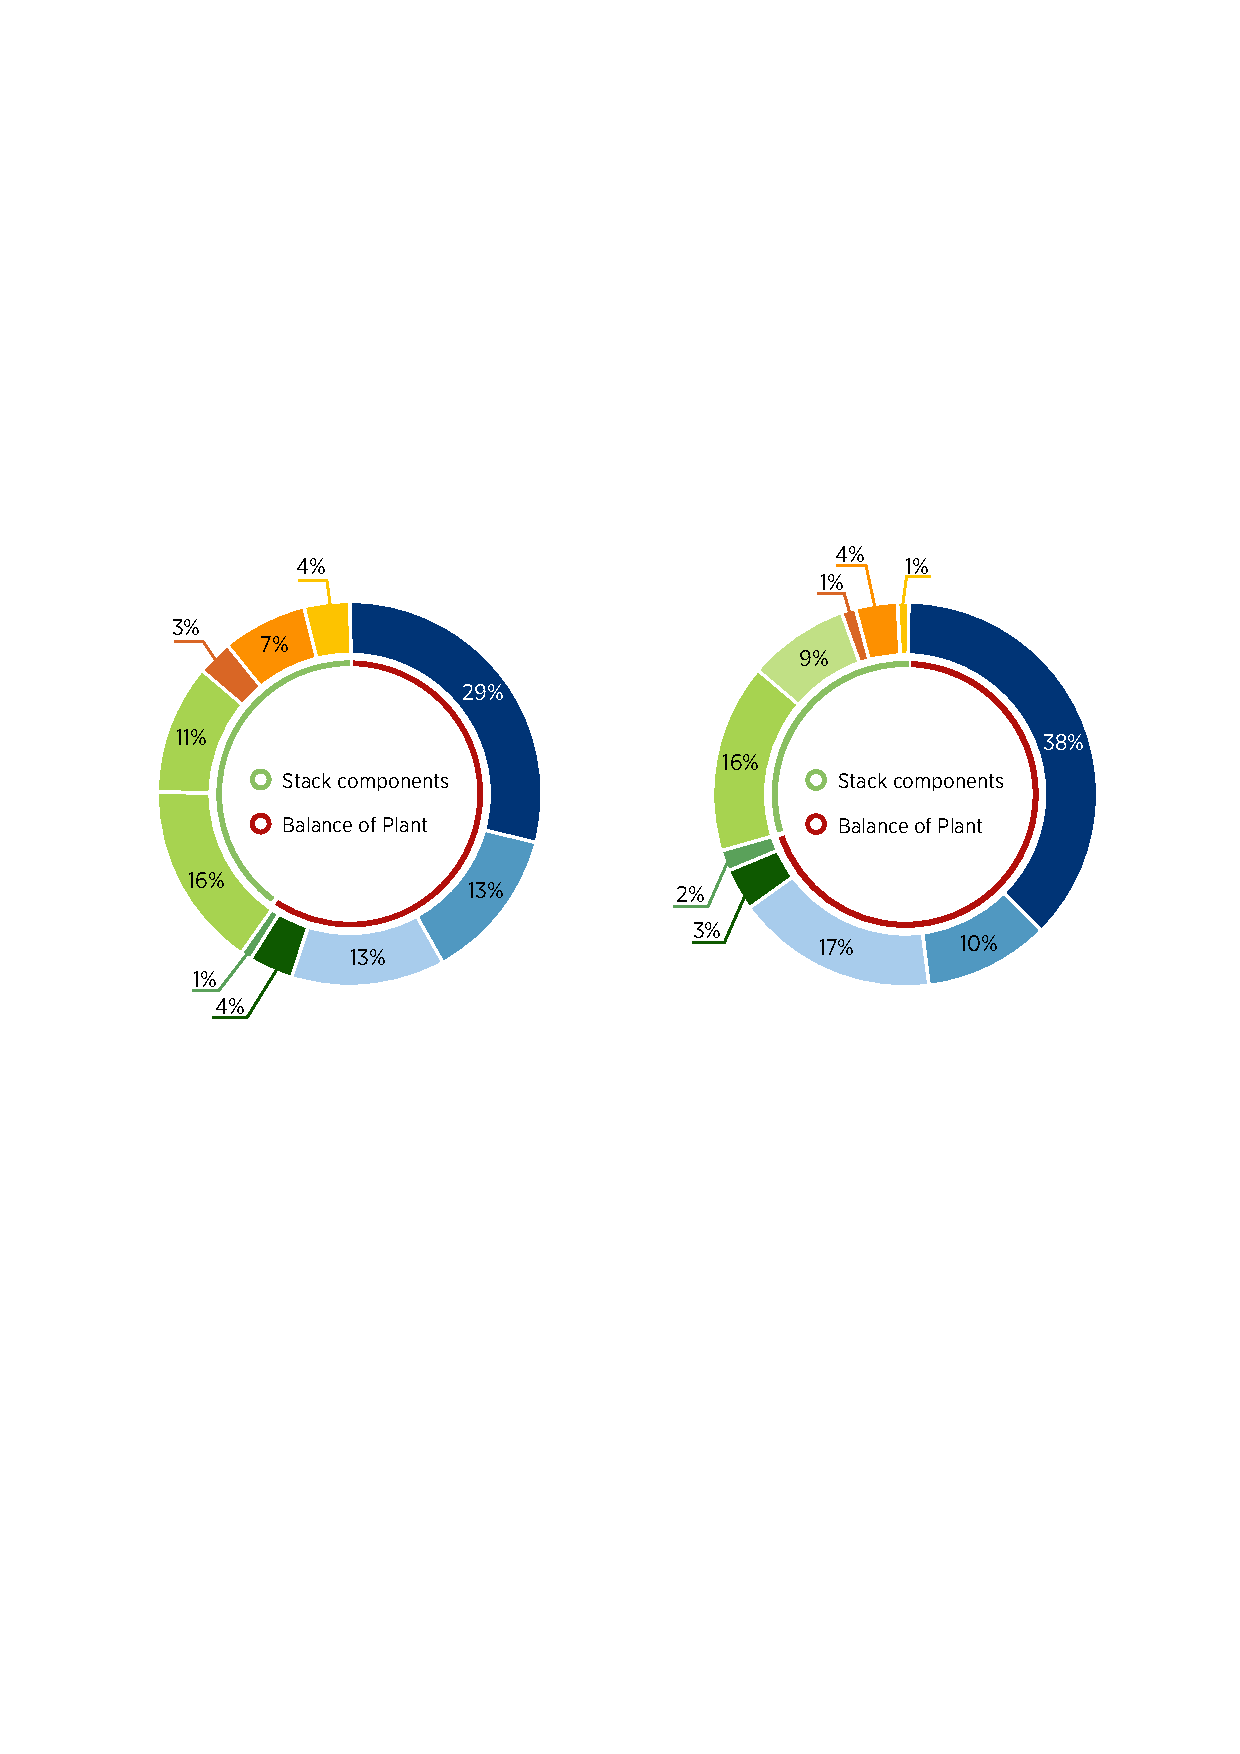
\includegraphics[width=0.7\linewidth]{content/Grafiken/ElyCost}
	\caption[Systemkosten PEM Elektrolyse]{Systemkosten \gls{PEM} Elektrolyse links 10 MW pro Jahr, rechts 1 GW pro Jahr \cite{IRENA2020}}
	\label{fig:elycost}
\end{figure}

Es zeigt sich in \ref{fig:elycapacity} darüber hinaus, dass der Ausbau der Elektrolyse in den letzten Jahren enorm gestiegen ist  und in Zukunft deutlich zunehmen wird. Die Weltweite Leistung ist gerade erst in den Gigawatt Bereich gestiegen und soll allein in Deutschland bis zum Jahr 2030 auf mindestens zehn Gigawatt ausgebaut werden.

\begin{figure}
	\centering
	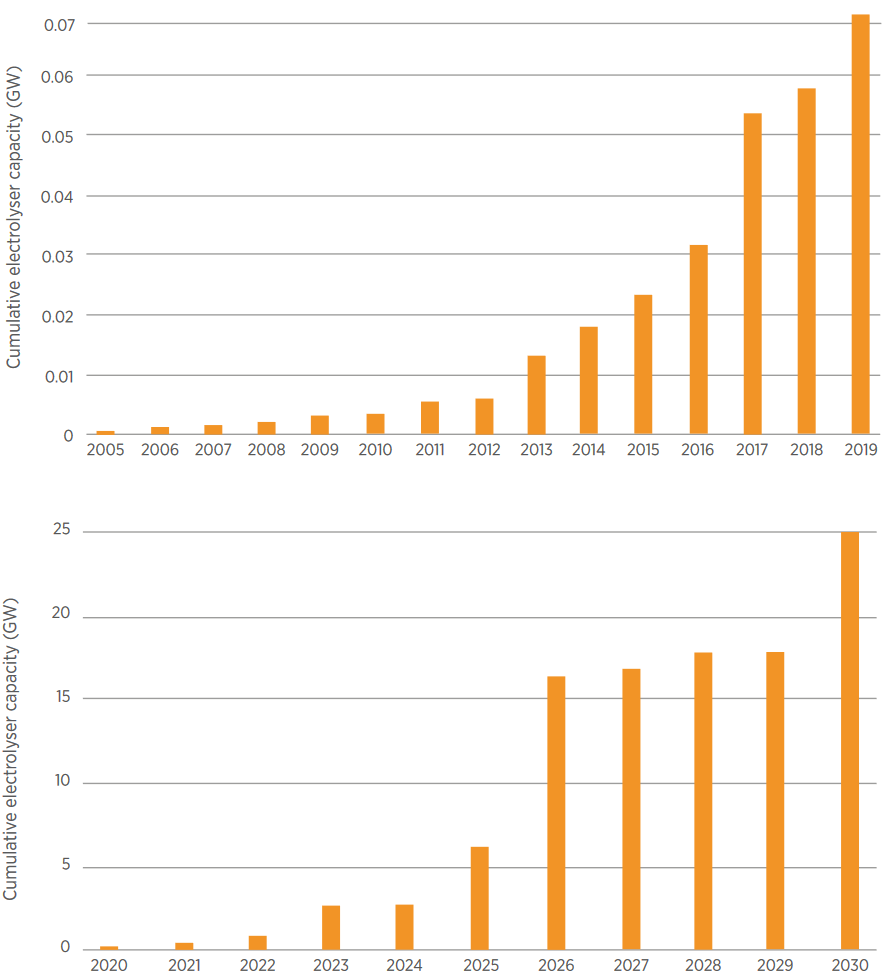
\includegraphics[width=0.7\linewidth]{content/Grafiken/Ely_Capacity}
	\caption[Elektrolyse Kapazität bis 2030]{Elektrolysekapazität Stand 2020 mit Ausblick bis 2030 \cite{IRENA2020}}
	\label{fig:elycapacity}
\end{figure}

Idiot  

\section{Ziel der Arbeit}
Ziel ist es die beiden vorab ausgewählten Stromrichter Topologien anhand von detaillierten Simulationen unter gegebenen Randbedingungen zu vergleichen, um eine eindeutige Bewertung durchzuführen. Dazu werden zunächst die Randbedingungen und Eigenschaften der Schnittstellen, Elektrolyseur und Stromnetz, definiert um diese in einer Simulation mittels Matlab und der Erweiterung PLECS abzubilden. Durch Modelle der Halbleiter kann die Verlustleistung und damit die Effizienz und indirekt der Kühlaufwand bewertet werden. Außerdem kann anhand der gespeicherten Energie in den Magnetischen Komponenten die Größe und Kosten dieser bewertet werden, da diese mit den größten Anteil an den Gesamtkosten für Stromrichter bilden. Weitere Komponenten wie Treiberschaltung und benötigte Kapazitäten spielen eine untergeordnete Rolle bei der Bewertung. Um die Bereitstellung von Systemdienstleistungen zu Berücksichtigen, wird die Verlustleistung bei einer Phasenverschiebung von 30 Grad und 0 Grad betrachtet. Anschließend soll eine Gesamtbewertung durch Gewichtungsfaktoren der einzelnen Kategorien erfolgen.